\documentclass{article}

\usepackage{graphicx}
\usepackage[hidelinks]{hyperref}
\usepackage{geometry}
\usepackage{amsmath}
\usepackage{listings}
\usepackage{wrapfig}

\geometry{
 a4paper,
 left=20mm,
 right=20mm,
 top=20mm,
 bottom=25mm,
}

\begin{document}

\begin{titlepage}
\begin{center}
\vspace*{1cm}
            
\Huge
\textbf{Assignment 2}
            
\vspace{1cm}

\Large
\text{Due: Monday, October 7, 2024}

\vspace{2cm}

\text{\texttt{Brian High}} \\
\text{\texttt{Thomas Hynes}} \\
\text{\texttt{Jeremy Middleman}} \\
\text{\texttt{Andrei Phelps}} \\
\text{\texttt{Wayne Rudnick}} \\

\vspace{2cm}


\includegraphics[scale=0.25]{../figs/icon.png}\\[0.5cm]

\vspace{9cm}

\textbf{CS 491/591: Neural Networks} \\

\end{center}
\end{titlepage}
\newpage

\section{How to Run the Program}
You can run the program by executing the main file using the python command.
\begin{verbatim}
    python main.py
\end{verbatim}

\section{Datasets} 
Two datasets were selected for this assignment: the Optical recognition of handwritten digits dataset and the Breast cancer wisconsin (diagnostic) dataset, both of which are Toy Datasets in the Scikit-Learn datasets library. The former has ten classes (from 1-10) and the latter has two classes (benign and malignant). The latter was selected because this is the only binary classification dataset that we could find in the scikit-learn toy and real-world datasets. The former was selected so that the accuracy of our models could be comopared when examining different combinations of numbers (i.e. 1 vs 2, 1, 7, etc.).

\section{Testing - Dataset #1, Digits}
\includegraphics[scale=0.75]{../figs/digitsTest.png} \\[0.5cm]

The first dataset we chose to test involved identifying which digit was displayed. Each digit had 64 features that our classification models used to recognize the digit. To make this a binary classification problem, we limited the classification to distinguishing between zeros and ones. We set a learning rate of 0.01 and ran 100 epochs for this test, using 288 samples as training data and 72 samples as test data.

Through testing, we found that the Weston Watkins SVM model and the Linear SVM model generally achieved the highest classification accuracy, often reaching 100 percent. We were not too surprised to see this as they utilize some of the same methods in order to classify samples. As expected, when we lowered the number of epochs, the accuracy of all classification models decreased. Conversely, increasing the number of epochs led to improved classification accuracy.

\section{Testing - Dataset 2, Breast Cancer}
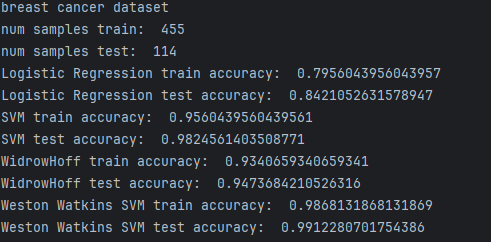
\includegraphics[scale=0.75]{../figs/BreastCancer.png} \\[0.5cm]

These tests yielded similar accuracy results results to the digits dataset. Logistic Regression performed the worse, Widrow Hoff was the second worst, SVM was the second best, and Weston Watkins was the best. The difference between Linear SVM and Weston Watkins accuracy was about the same for the first data set. In this test we can see that some classifier models work better with certain classification requests than others.


\section{Individual Contributions}

\subsection{Brian High}
\begin{itemize}
    \item[1)] Implemented Logistic regression
\end{itemize}

\subsection{Thomas Hynes}
\begin{itemize}
    \item[1)] Wrote the python class for Widrow Hoff.
    \item[2)] Added comments to code files.
\end{itemize}

\subsection{Jeremy Middleman}
\begin{itemize}
    \item[1)] Worked on implementing test cases, including writing a lot of the main class.
    \item[2)] Helped with the report
\end{itemize}

\subsection{Andrei Phelps}
\begin{itemize}
    \item[1)] Implemented the Weston-Watkins SVM for Part 3.
    \item[2)] Ensured the Weston-Watkins SVM was capable of multi-class classification for Part 4. 
\end{itemize}

\subsection{Wayne Rudnick}
\begin{itemize}
    \item[1)] Wrote the python class for Linear Support Vector Machine
    \item[2)] Assisted with part 2 in creating the tests for our 4 classification methods
    \item[3)] Fixed and Revamped Widrow-Hoff to return a binary classification and resolved overflow issues within the class
    \item[4)] Worked with Jeremy on creating the report
\end{itemize}

\end{document}
